\documentclass{article}

\usepackage{amsmath}

\usepackage{booktabs}
\usepackage{multirow}
\usepackage{xcolor}
\usepackage{graphicx}
\usepackage{colortbl}

\usepackage{titling}
\predate{}
\postdate{}
\date{}

\title{SAT Competition 2023}
\author{Markus Iser}

\begin{document}
\maketitle

Evaluation is based on solver runtimes in SAT Competition 2023 without the checker-timeout penalty 
in order to compare the pure proof-production performance of solvers.

At the same time, this is a sample document for testing and showing 
how to use the evaluation functions in this repository.

\section{CDF and Cactus Plots}

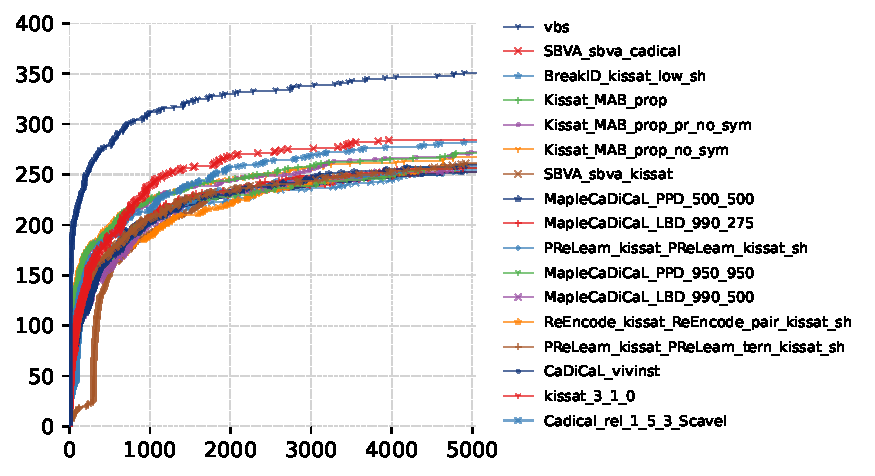
\includegraphics{gen/sc2023/cdf.pdf}
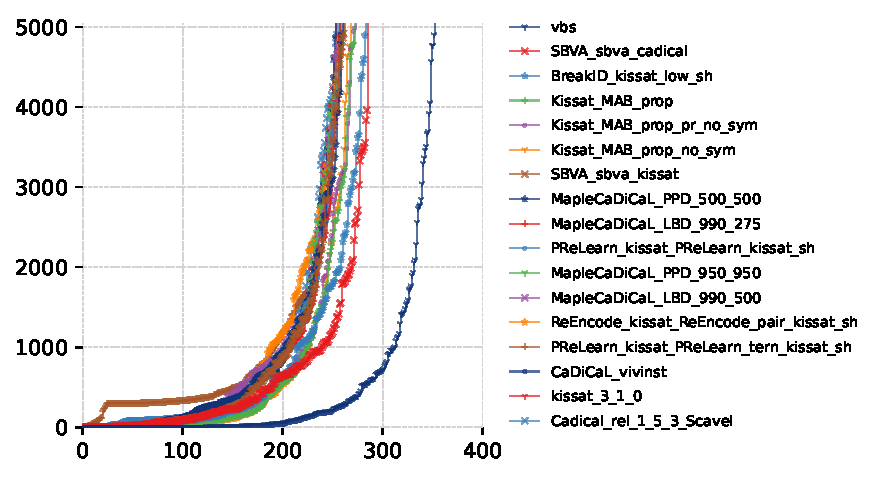
\includegraphics{gen/sc2023/cactus.pdf}


\section{SBVA-CaDiCaL vs. SBVA-Kissat}

\begin{tabular}{lr|cc|c}
\toprule
Family & Count & SBVA CaDiCaL & SBVA Kissat & VBS \\
\midrule
Miscellaneous & 70 & 3071.07 & \bfseries 2779.72 & 2356.70 \\
Argumentation & 20 & 3693.93 & \bfseries 3477.05 & 3475.19 \\
Profitable-Robust-Production & 20 & \bfseries 2470.42 & 5058.18 & 2469.91 \\
Social-Golfer & 20 & \bfseries 7555.16 & 7690.23 & 7533.95 \\
Cryptography-Ascon & 20 & \bfseries 356.82 & 2811.89 & 324.37 \\
Set-Covering & 20 & 722.01 & \bfseries 345.13 & 238.27 \\
Hashtable-Safety & 20 & \bfseries 797.46 & 1396.84 & 797.46 \\
Interval-Matching & 20 & \bfseries 10000.00 & \bfseries 10000.00 & 10000.00 \\
Register-Allocation & 20 & 101.20 & \bfseries 95.28 & 61.05 \\
School-Timetabling & 19 & \bfseries 1399.65 & 2178.28 & 1187.72 \\
Brent-Equations & 19 & \bfseries 232.86 & 404.04 & 153.79 \\
Cryptography-Simon & 17 & \bfseries 10000.00 & \bfseries 10000.00 & 10000.00 \\
Grs-Fp-Comm & 17 & \bfseries 3649.90 & 4088.89 & 3647.53 \\
Satcoin & 15 & \bfseries 1395.53 & 10000.00 & 1395.53 \\
Mutilated-Chessboard & 12 & \bfseries 3194.54 & 4228.03 & 3194.54 \\
Tseitin & 11 & \bfseries 8196.91 & 8213.62 & 8196.74 \\
Miter & 11 & \bfseries 3134.91 & 4032.27 & 3105.64 \\
Pigeon-Hole & 8 & 5261.85 & \bfseries 5168.71 & 5168.70 \\
Hardware-Verification & 8 & 2832.05 & \bfseries 2714.99 & 2705.49 \\
Cryptography & 7 & 1578.46 & \bfseries 330.68 & 316.73 \\
Planning & 6 & \bfseries 6.97 & 7.75 & 6.49 \\
Quasigroup-Completion & 5 & 9.33 & \bfseries 6.49 & 6.12 \\
Reg-N & 5 & \bfseries 10000.00 & \bfseries 10000.00 & 10000.00 \\
Subsumptiontest & 5 & \bfseries 230.22 & 278.97 & 230.22 \\
Or\_Randxor & 5 & \bfseries 21.82 & 22.94 & 17.87 \\
\hline All & 400 & \bfseries 3257.62 & 3882.65 & 3051.46 \\
\bottomrule
\end{tabular}


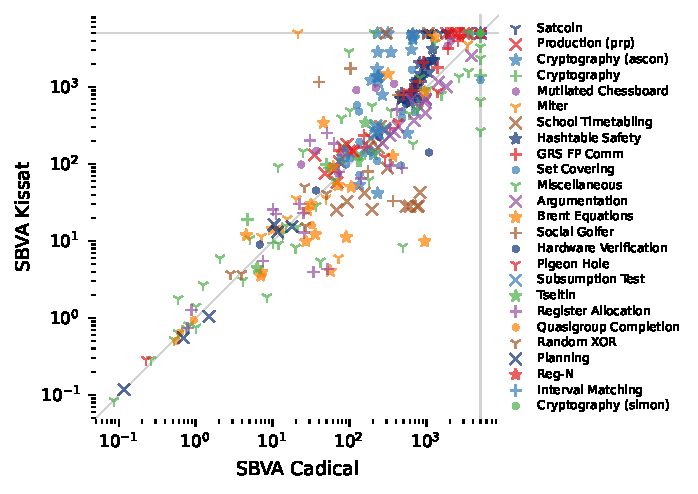
\includegraphics{gen/sc2023/sbva_cadical_kissat_logscale.pdf}

\section{CaDiCaL-vivinst vs. Kissat-3.1.0}

\begin{tabular}{lr|cc|c}
\toprule
Family & Count & Cadical\_Vivinst & Kissat\_3\_1\_0 & VBS \\
\midrule
Satcoin & 15 & 7388.71 & \bfseries 2495.86 & 2129.11 \\
Profitable-Robust-Production & 20 & \bfseries 2463.60 & 5024.62 & 2458.96 \\
Mutilated-Chessboard & 12 & \bfseries 2933.52 & 4131.55 & 2932.48 \\
Register-Allocation & 20 & \bfseries 8998.24 & 10000.00 & 8998.24 \\
Miter & 11 & \bfseries 3149.19 & 3710.41 & 3109.62 \\
School-Timetabling & 19 & \bfseries 1264.86 & 1669.03 & 1141.51 \\
Miscellaneous & 70 & 3140.29 & \bfseries 2779.33 & 2601.18 \\
Hashtable-Safety & 20 & \bfseries 460.96 & 805.04 & 458.63 \\
Social-Golfer & 20 & 7871.79 & \bfseries 7565.89 & 7564.08 \\
Grs-Fp-Comm & 17 & \bfseries 3659.80 & 3864.28 & 3632.29 \\
Argumentation & 20 & 3688.69 & \bfseries 3597.93 & 3566.72 \\
Set-Covering & 20 & 259.73 & \bfseries 174.42 & 149.20 \\
Pigeon-Hole & 8 & 6502.28 & \bfseries 6425.97 & 6412.68 \\
Cryptography-Ascon & 20 & 378.92 & \bfseries 303.29 & 284.36 \\
Brent-Equations & 19 & \bfseries 176.54 & 249.81 & 137.45 \\
Hardware-Verification & 8 & 2893.13 & \bfseries 2831.85 & 2755.54 \\
Cryptography & 7 & \bfseries 1602.26 & 1638.69 & 1582.76 \\
Subsumptiontest & 5 & \bfseries 46.47 & 76.98 & 25.46 \\
Tseitin & 11 & \bfseries 8201.03 & 8214.31 & 8199.91 \\
Planning & 6 & 13.03 & \bfseries 8.63 & 6.66 \\
Quasigroup-Completion & 5 & 2.70 & \bfseries 1.91 & 1.91 \\
Reg-N & 5 & \bfseries 10000.00 & \bfseries 10000.00 & 10000.00 \\
Interval-Matching & 20 & \bfseries 10000.00 & \bfseries 10000.00 & 10000.00 \\
Cryptography-Simon & 17 & \bfseries 10000.00 & \bfseries 10000.00 & 10000.00 \\
Or\_Randxor & 5 & \bfseries 10000.00 & \bfseries 10000.00 & 10000.00 \\
\hline All & 400 & \bfseries 4048.63 & 4050.74 & 3709.67 \\
\bottomrule
\end{tabular}

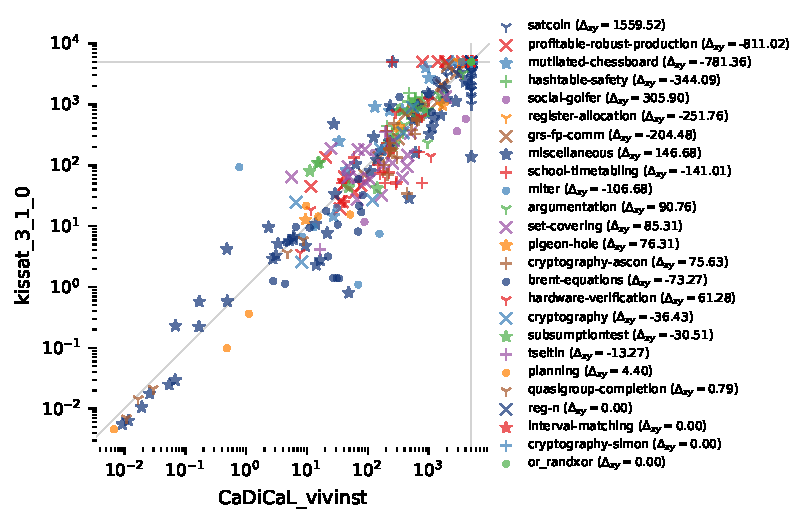
\includegraphics{gen/sc2023/Cadical_vivinst_Kissat_310_logscale.pdf}

\section{SBVA-CaDiCaL vs. BreakId}

\begin{tabular}{lr|cc|c}
\toprule
Family & Count & SBVA CaDiCaL & Breakid\_Kissat\_Low\_Sh & VBS \\
\midrule
Miscellaneous & 70 & 3071.07 & \bfseries 1964.08 & 1245.85 \\
Argumentation & 20 & 3693.93 & \bfseries 3447.39 & 3446.95 \\
Profitable-Robust-Production & 20 & \bfseries 2470.42 & 5031.37 & 2460.03 \\
Social-Golfer & 20 & \bfseries 7555.16 & 9013.05 & 7548.93 \\
Cryptography-Ascon & 20 & \bfseries 356.82 & 800.41 & 297.61 \\
Set-Covering & 20 & 722.01 & \bfseries 262.39 & 188.29 \\
Hashtable-Safety & 20 & \bfseries 797.46 & 1700.77 & 789.68 \\
Interval-Matching & 20 & \bfseries 10000.00 & \bfseries 10000.00 & 10000.00 \\
Register-Allocation & 20 & \bfseries 101.20 & 892.52 & 42.72 \\
School-Timetabling & 19 & \bfseries 1399.65 & 2371.42 & 1234.90 \\
Brent-Equations & 19 & \bfseries 232.86 & 698.16 & 168.16 \\
Cryptography-Simon & 17 & \bfseries 10000.00 & \bfseries 10000.00 & 10000.00 \\
Grs-Fp-Comm & 17 & \bfseries 3649.90 & 3865.34 & 3638.10 \\
Satcoin & 15 & \bfseries 1395.53 & 1421.87 & 1370.56 \\
Mutilated-Chessboard & 12 & \bfseries 3194.54 & 4240.09 & 3194.54 \\
Tseitin & 11 & 8196.91 & \bfseries 5772.63 & 5764.96 \\
Miter & 11 & \bfseries 3134.91 & 3143.29 & 3118.73 \\
Pigeon-Hole & 8 & 5261.85 & \bfseries 5128.03 & 5128.03 \\
Hardware-Verification & 8 & \bfseries 2832.05 & 2865.77 & 2717.96 \\
Cryptography & 7 & 1578.46 & \bfseries 1570.64 & 1554.56 \\
Planning & 6 & \bfseries 6.97 & 10.98 & 6.96 \\
Quasigroup-Completion & 5 & 9.33 & \bfseries 3.43 & 3.43 \\
Reg-N & 5 & \bfseries 10000.00 & \bfseries 10000.00 & 10000.00 \\
Subsumptiontest & 5 & 230.22 & \bfseries 89.14 & 89.14 \\
Or\_Randxor & 5 & \bfseries 21.82 & 103.93 & 21.82 \\
\hline All & 400 & \bfseries 3257.62 & 3376.88 & 2805.19 \\
\bottomrule
\end{tabular}

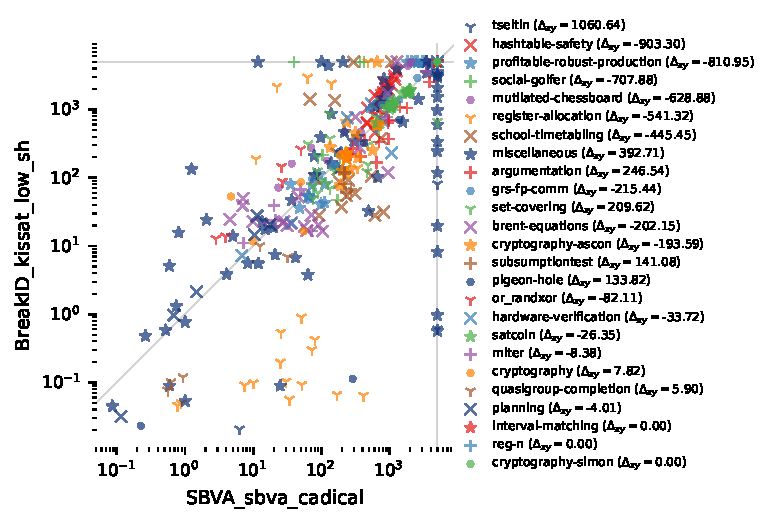
\includegraphics{gen/sc2023/sbva_cadical_breakid_logscale.pdf}


\section{Family-wise CDF Plots}

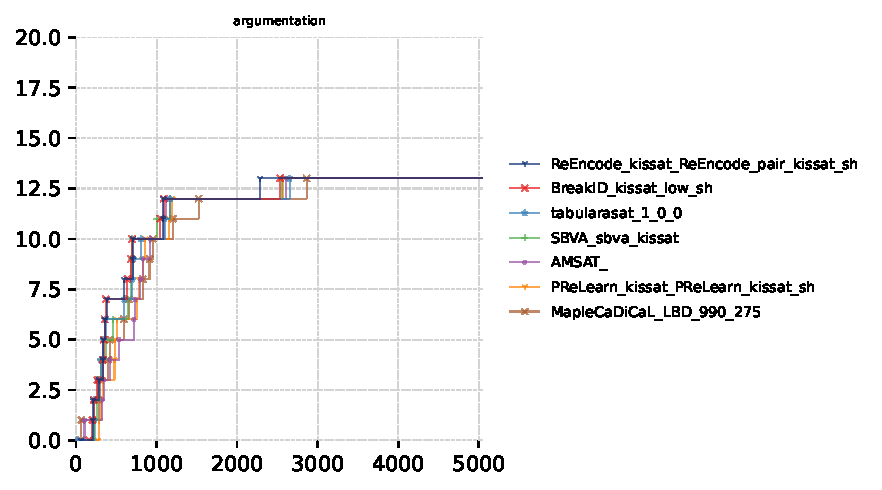
\includegraphics[width=\linewidth]{gen/sc2023/cdfs/cdf-argumentation.pdf}
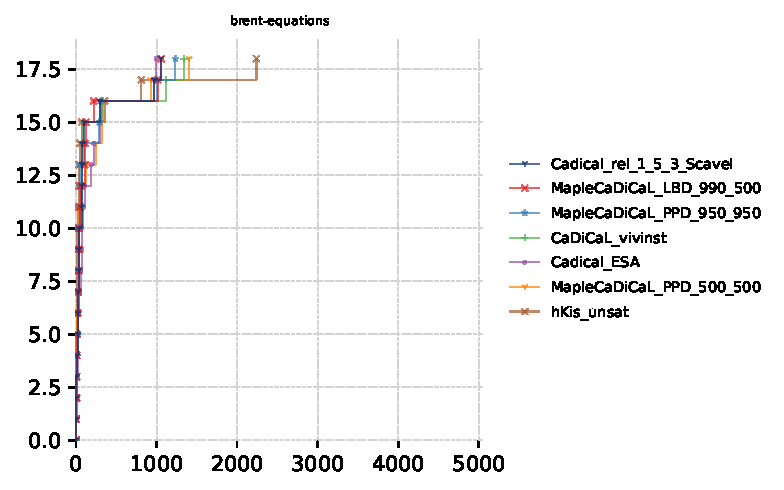
\includegraphics[width=\linewidth]{gen/sc2023/cdfs/cdf-brent-equations.pdf}
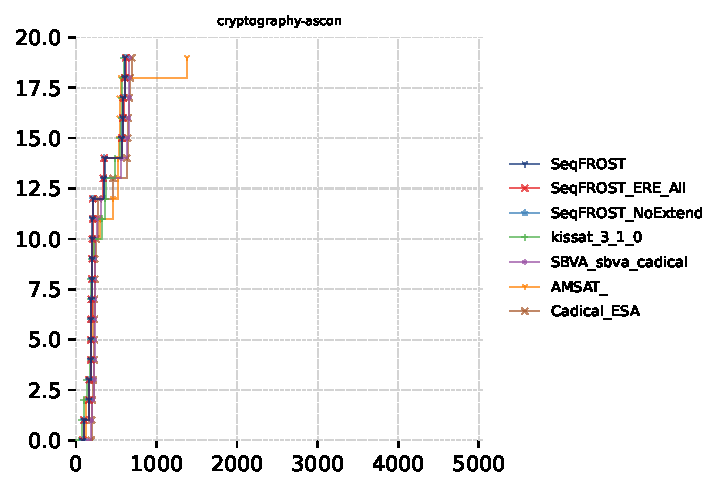
\includegraphics[width=\linewidth]{gen/sc2023/cdfs/cdf-cryptography-ascon.pdf}
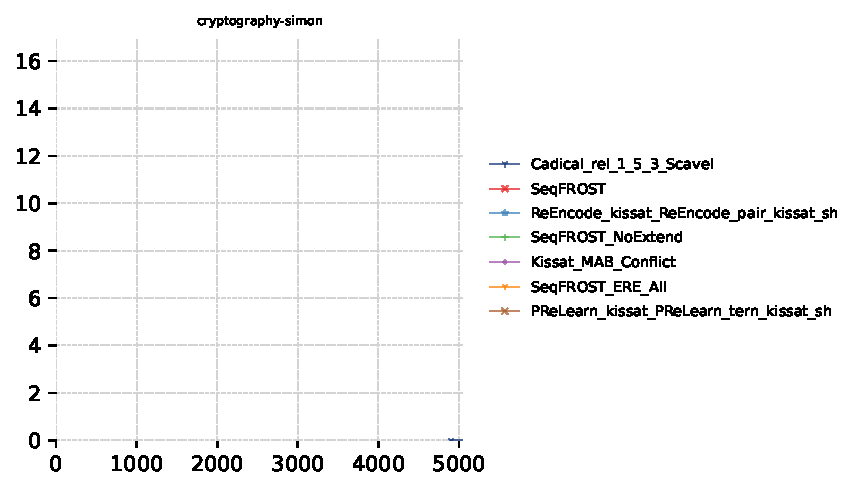
\includegraphics[width=\linewidth]{gen/sc2023/cdfs/cdf-cryptography-simon.pdf}
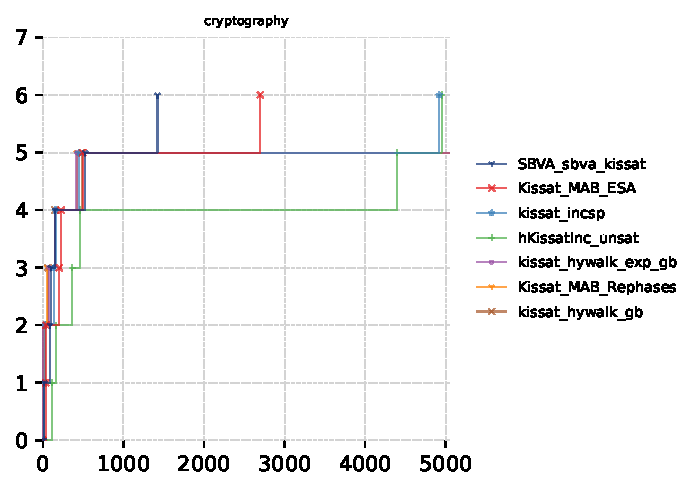
\includegraphics[width=\linewidth]{gen/sc2023/cdfs/cdf-cryptography.pdf}
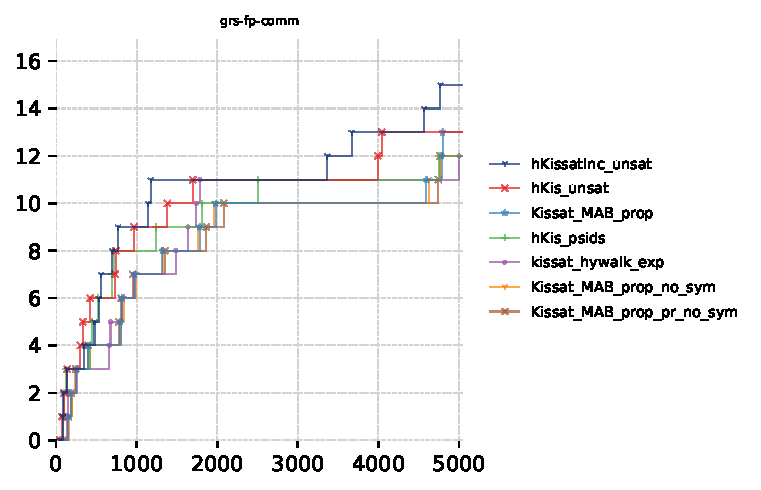
\includegraphics[width=\linewidth]{gen/sc2023/cdfs/cdf-grs-fp-comm.pdf}
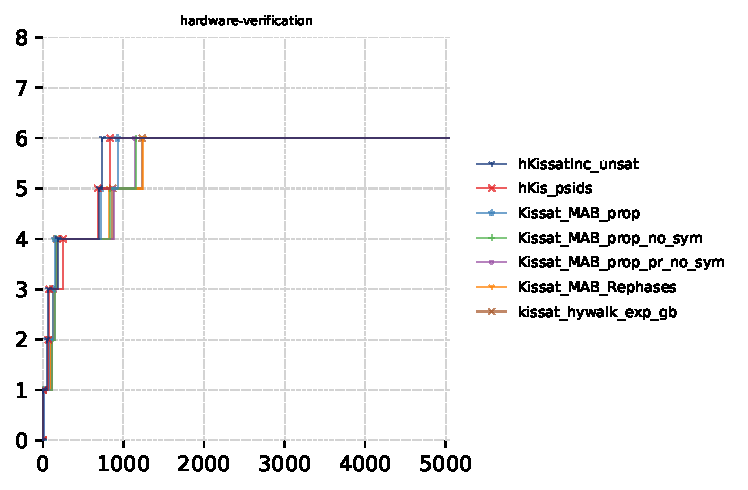
\includegraphics[width=\linewidth]{gen/sc2023/cdfs/cdf-hardware-verification.pdf}
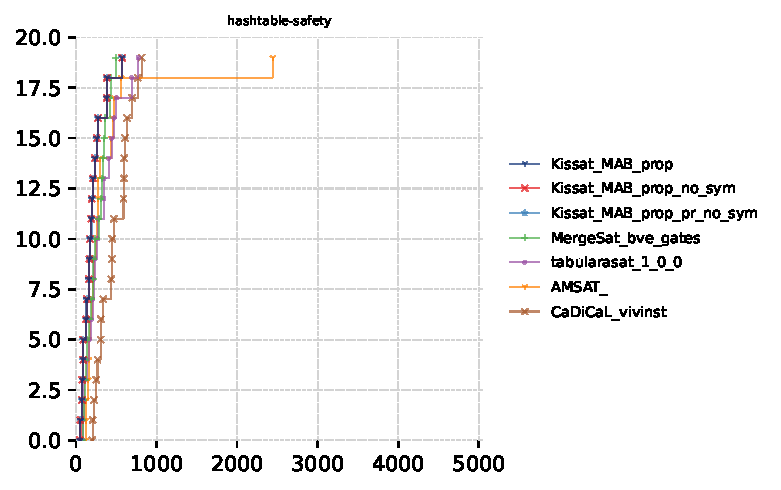
\includegraphics[width=\linewidth]{gen/sc2023/cdfs/cdf-hashtable-safety.pdf}
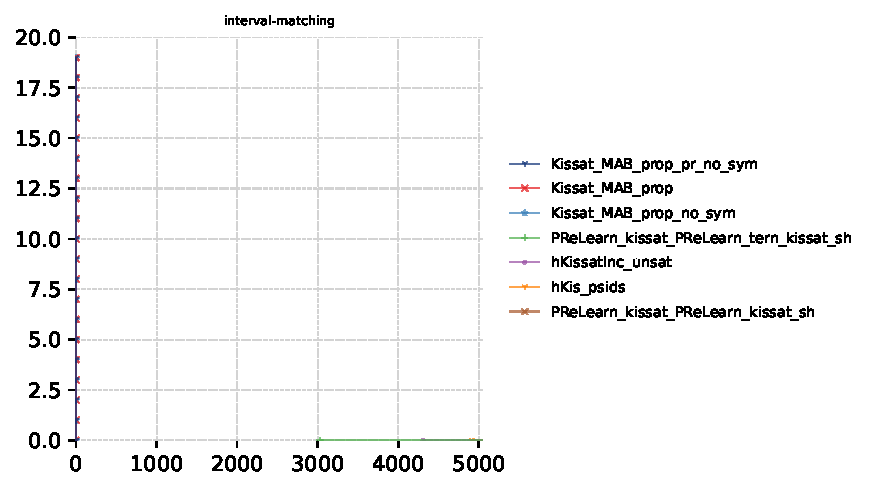
\includegraphics[width=\linewidth]{gen/sc2023/cdfs/cdf-interval-matching.pdf}
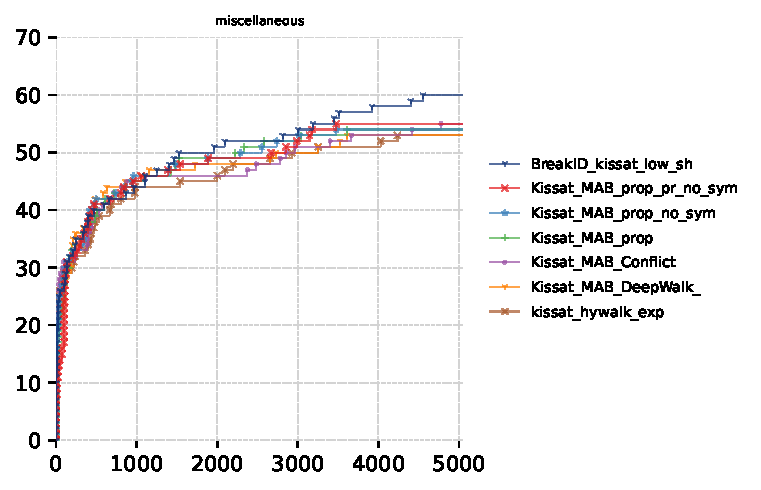
\includegraphics[width=\linewidth]{gen/sc2023/cdfs/cdf-miscellaneous.pdf}
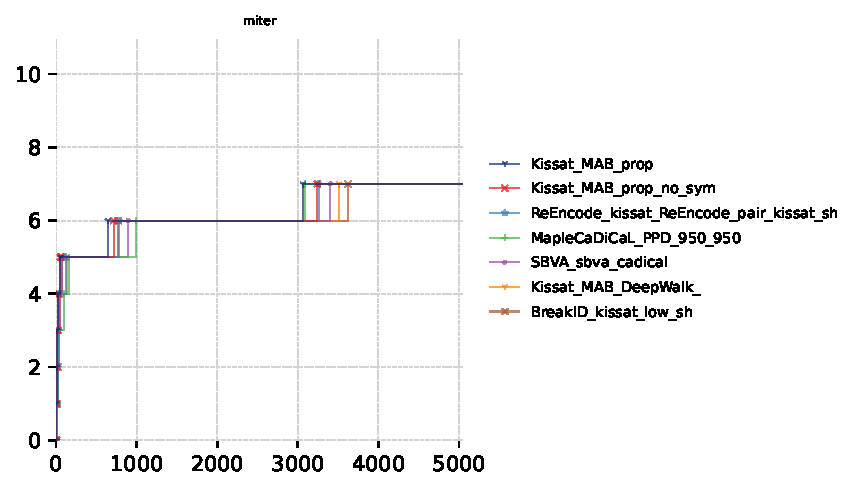
\includegraphics[width=\linewidth]{gen/sc2023/cdfs/cdf-miter.pdf}
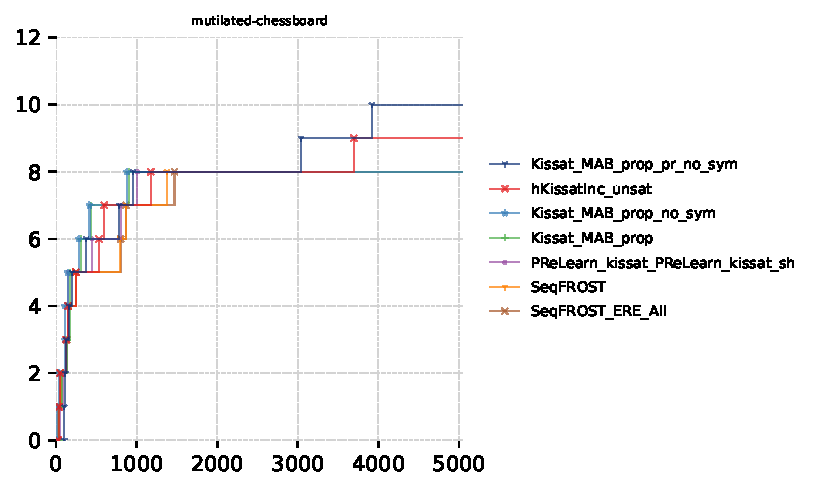
\includegraphics[width=\linewidth]{gen/sc2023/cdfs/cdf-mutilated-chessboard.pdf}
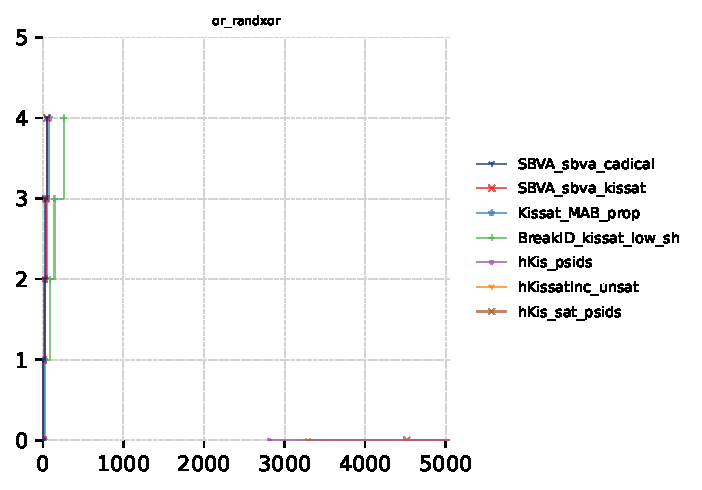
\includegraphics[width=\linewidth]{gen/sc2023/cdfs/cdf-or_randxor.pdf}
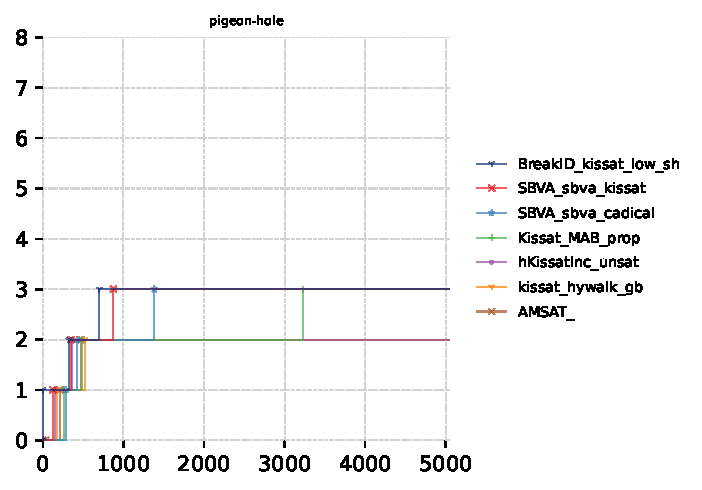
\includegraphics[width=\linewidth]{gen/sc2023/cdfs/cdf-pigeon-hole.pdf}
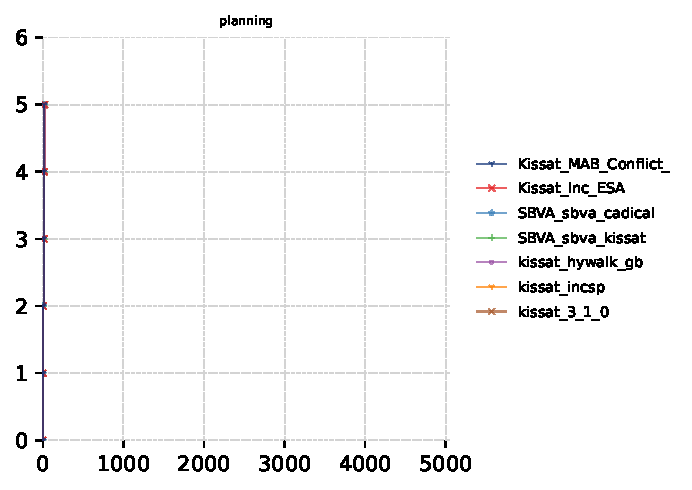
\includegraphics[width=\linewidth]{gen/sc2023/cdfs/cdf-planning.pdf}
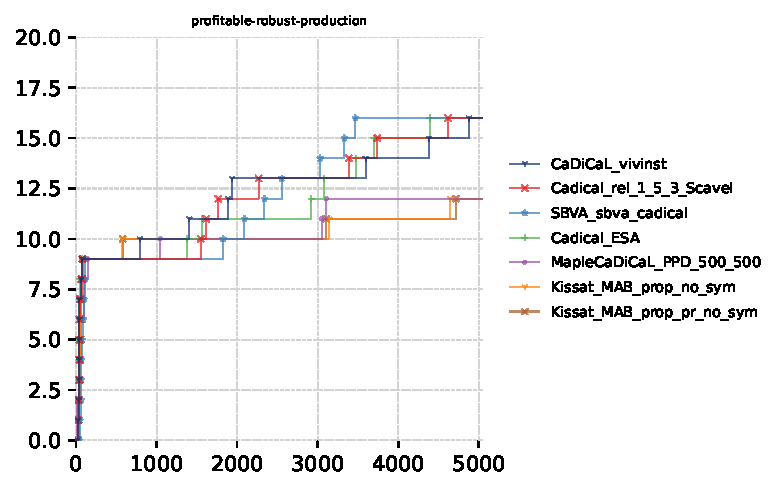
\includegraphics[width=\linewidth]{gen/sc2023/cdfs/cdf-profitable-robust-production.pdf}
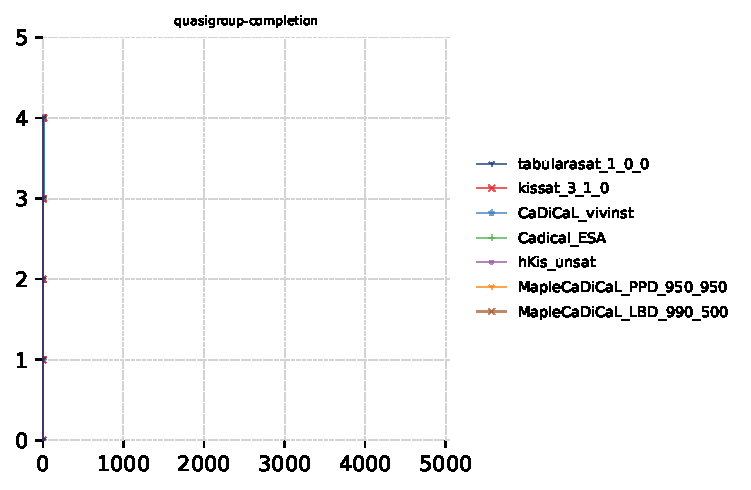
\includegraphics[width=\linewidth]{gen/sc2023/cdfs/cdf-quasigroup-completion.pdf}
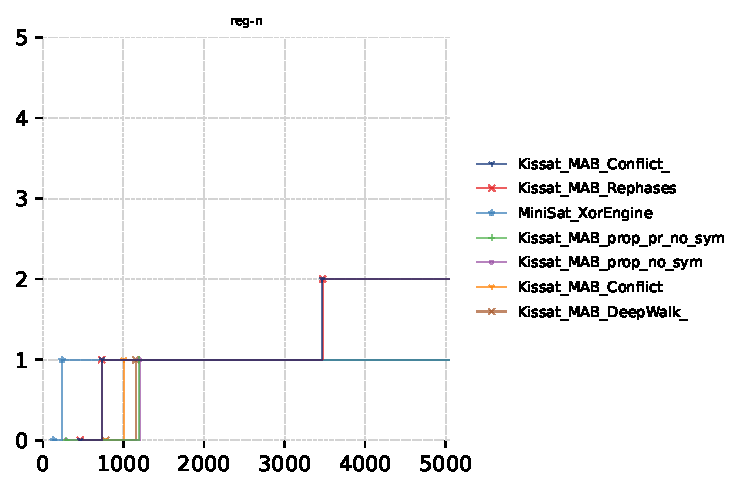
\includegraphics[width=\linewidth]{gen/sc2023/cdfs/cdf-reg-n.pdf}
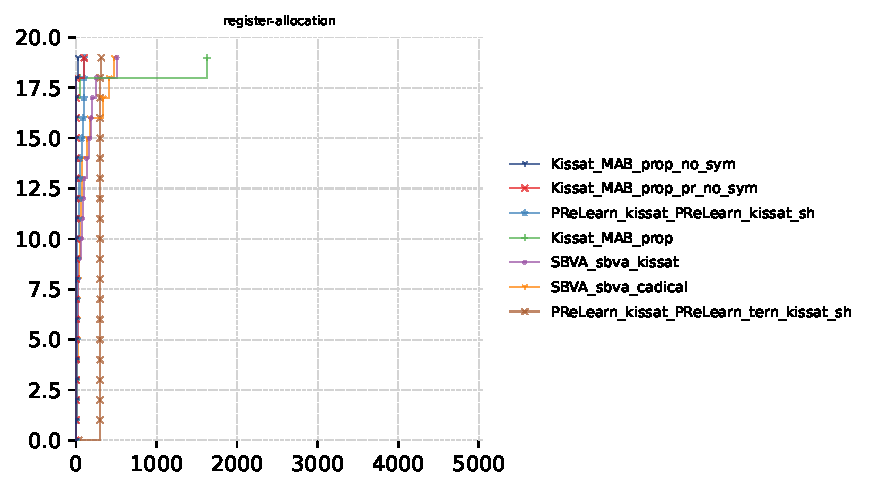
\includegraphics[width=\linewidth]{gen/sc2023/cdfs/cdf-register-allocation.pdf}
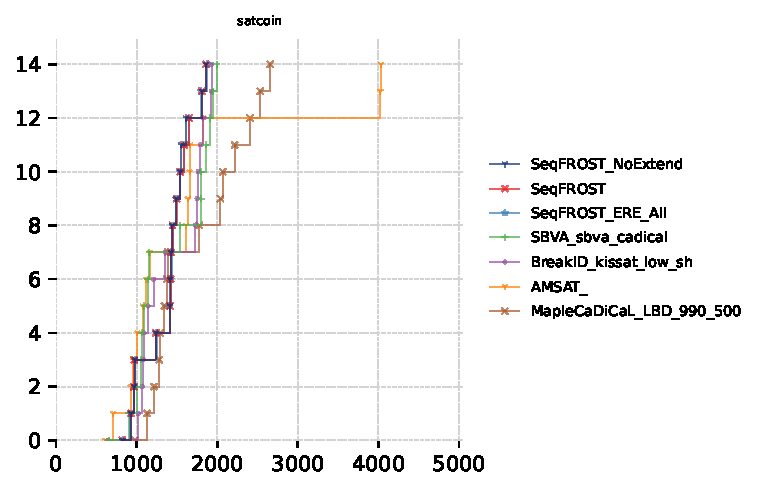
\includegraphics[width=\linewidth]{gen/sc2023/cdfs/cdf-satcoin.pdf}
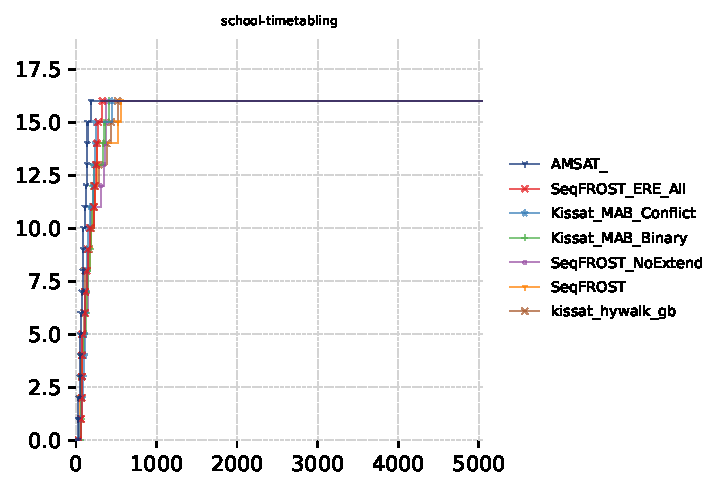
\includegraphics[width=\linewidth]{gen/sc2023/cdfs/cdf-school-timetabling.pdf}
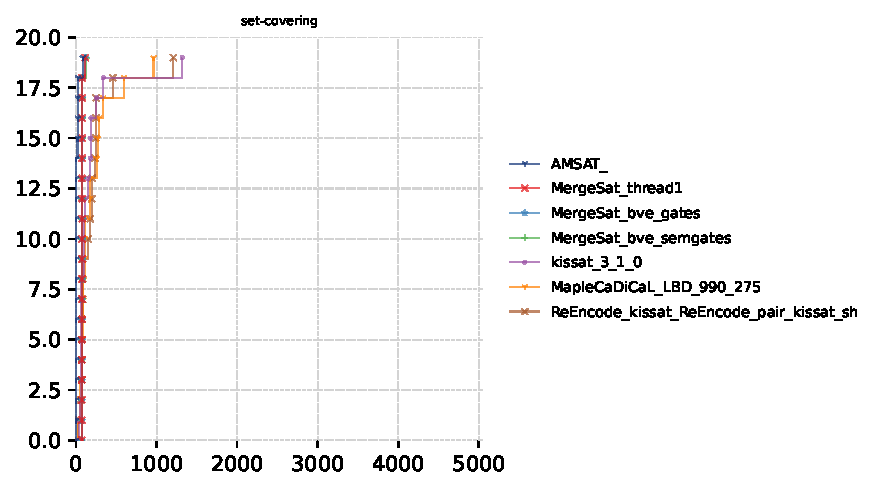
\includegraphics[width=\linewidth]{gen/sc2023/cdfs/cdf-set-covering.pdf}
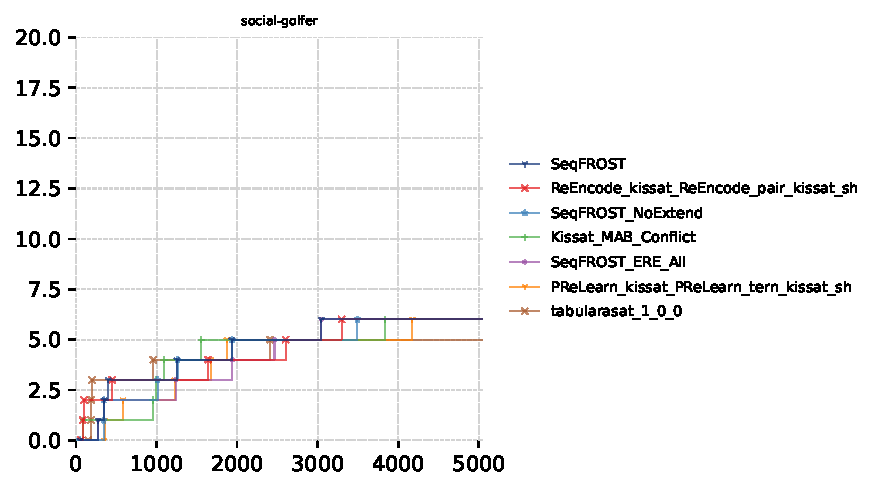
\includegraphics[width=\linewidth]{gen/sc2023/cdfs/cdf-social-golfer.pdf}
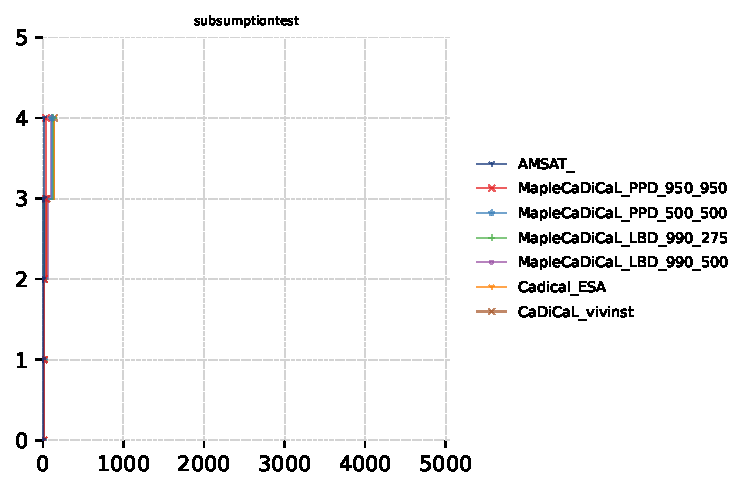
\includegraphics[width=\linewidth]{gen/sc2023/cdfs/cdf-subsumptiontest.pdf}
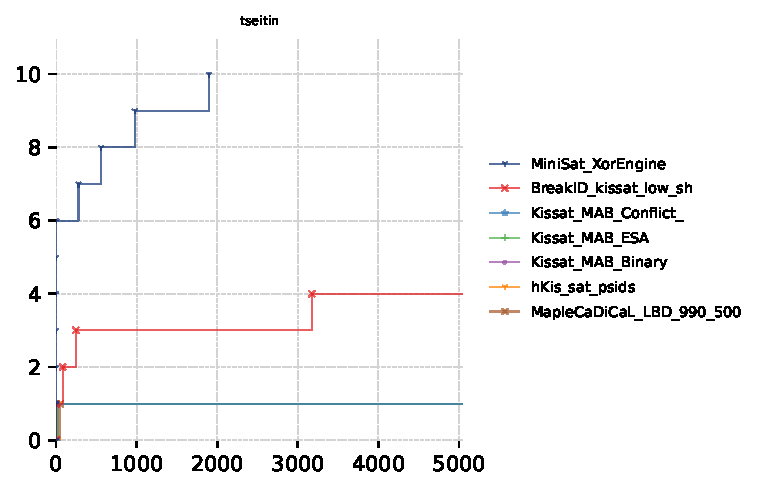
\includegraphics[width=\linewidth]{gen/sc2023/cdfs/cdf-tseitin.pdf}


\end{document}